\chapter{Tests}
\label{chap:tests}

\section{Tests outline}

Two kinds of tests examining different sides of solution are performed:
\begin{itemize}
  \item performance tests -- laboratory tests examining designed solution's performance in various conditions
  \item psychoacoustic test -- experiment examining audibility of signal hidden by presented solution
\end{itemize}

\noindent In every type of test, synthesis\,/\,analysis algorithms are parameterized with following values:

\begin{itemize}
  \item byte duration = 200\,ms
  \item carrier signal band = 8000--8800\,\mbox{Hz}
\end{itemize}

With this setup, the solution achieves effective data bandwidth of 26.66\,\mbox{bps} (bits per second).

Unfortunately tests are not performed on mobile platform because of longer time required for implementation. All performance tests 
are conducted in acoustic laboratory using stationary devices.

\section{Performance tests}
\subsection{Overview}
The purpose of performance tests is to examine the possibilities of implemented solution. Information about algorithm effectiveness is expected as an procedure output.
Performance tests are conducted in a laboratory environment to enable environment manipulation.
To get most informative output data and effective testing environment, following features are required:
\begin{itemize}
  \item value-neutrality -- any kind of unwanted environmental noise is eliminated
  \item versatility -- various environment conditions are simulated
  \item repeatability -- tests are easy to conduct and repeat many times in the same form.
\end{itemize}

To fulfill the requirements, anechoic chamber and professional recording\,/\,playback facilities are employed.
See Figure \ref{fig:test-environment} for block diagram of test environment setup.

\clearpage

\subsection{Environment setup}
\begin{figure}[h]
  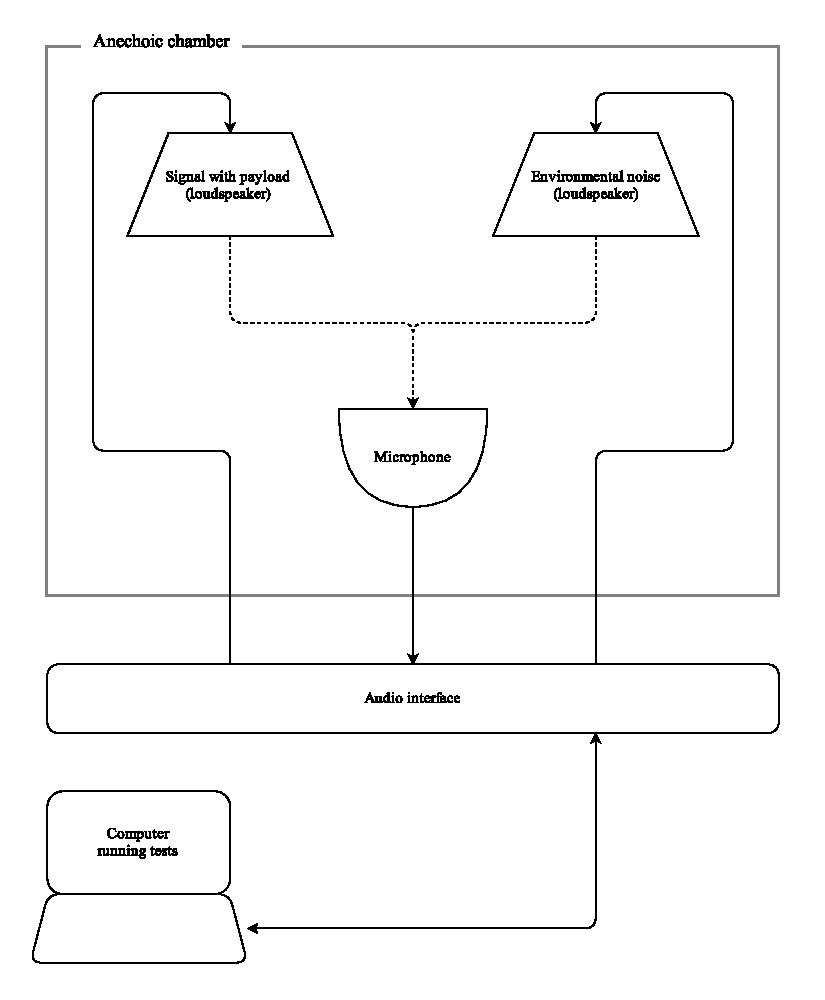
\includegraphics[width=\linewidth]{figures/experiments/environment}
  \caption{Test environment diagram}
  \label{fig:test-environment}
\end{figure}
Two loudspeakers are directed to microphone in monophonic mode. Microphone output is connected to audio interface input. Loudspeakers are connected to separate
interface outputs. Computer plays encoded signal on one speaker and environmental noise on the other one. At the same time, audio signal is
recorded using the microphone. Recorded samples are then analyzed using developed solution. The decoded payload is compared to original and Bit Error Rate (BER) is computed.

\clearpage

Following equipment is used to realize described solution:
\begin{itemize}
\item 2 $\times$ Tannoy 800A Active monitor loudspeakers
\item Shure VP88 MS-stereo-condenser microphone
\item Focusrite Scarlett 18i20 USB Audio interface
\item MacBook Air with OS X Yosemite (10.9)
\end{itemize}

\subsection{Implementation}

Test software is implemented in python programming language, like the algorithm library. The language was chosen to stay consistent across entire solution.
It is also easy to utilize encoding\,/\,decoding library written in the same language.
The \verb|Experiment| class is responsible for conducting performance tests.

Public methods:
\begin{itemize}
  \item \verb|Experiment(host, noise, host_db, noise_db, payload)|
    Constructor

    Arguments:
    \begin{itemize}
      \item \verb|host|\quad host signal file path (\verb|string|)
      \item \verb|noise|\quad noise signal file path (\verb|string|)
      \item \verb|host_db|\quad amplitude of host signal in \mbox{dB} (\verb|float|)
      \item \verb|noise_db|\quad amplitude of noise signal in \mbox{dB} (\verb|float|)
      \item \verb|payload|\quad bytes to be transmitted (list of \verb|int|)
    \end{itemize}

  \item \verb|run()|

    When this method is called, experiment procedure starts. After conducted experiment, all parameters with decoded payload are appended in python format to \verb|experiment_output.txt| file.

    Return value: \verb|decoded_payload|
    \begin{itemize}
    \item \verb|decoded_payload| – payload decoded from recorded sample (array of \verb|int|)
    \end{itemize}

  \item \verb|BER(correct, computed)|

    Static class method.
    It reckons bit error rate for decoded payload data.

    Arguments:
    \begin{itemize}
      \item \verb|correct| -- original payload (array of \verb|int|)
      \item \verb|computed| -- decoded payload (array of \verb|int|)
    \end{itemize}

    Return value: \verb|bit_error_rate|
    \begin{itemize}
      \item \verb|bit_error_rate| -- reckoned bit error rate
    \end{itemize}

\end{itemize}

See Figure \ref{fig:experiment-application} for example usage of \verb|Experiment| class in an application.
\begin{figure}[h]
  \centering
  \inputminted[linenos]{python}{listings/experiment_example.py}
  \caption{Example usage of experiment class in an application}
  \label{fig:experiment-application}
\end{figure}

\subsection{Sound samples}
\label{subsec:sound-samples}
Two types of sound samples are needed to conduct performance tests:
\begin{itemize}
  \item host samples -- three sampled pieces of music to host encoded payload
  \item noise samples -- four various environmental noises
\end{itemize}
All audio samples used in tests are 24-bit monophonic WAV files. All spectrum charts have red-marked region in frequency range
used by presented solution. In case of noise signals -- they should disturb decoding process as much as there is power in this range.

\subsubsection{Noise samples}
All environmental noise is recorded especially for the purpose of the project. From many recorded sounds, only
three probes were selected. The selection is based on spectral analysis. Only sound samples containing much power in carrier signal
band are used.
Following four pieces were selected:
\begin{itemize}
  \item \verb|ambulance.wav| -- ambulance emergency signal (See: Figure \ref{fig:ambulance-analysis})
  \item \verb|bottle-scratch.wav| -- sound of scraping glass bottles (See: Figure \ref{fig:bottle-scratch-analysis})
  \item \verb|crowd.wav| -- speaking crowd (See: Figure \ref{fig:crowd-analysis})
  \item \verb|keys.wav| -- clanking keys (See: Figure \ref{fig:keys-analysis})
\end{itemize}


\noindent To record these sounds following equipment has been used:
\begin{itemize}
  \item Tascam DR-40 Linear PCM hand-recorder
  \item Shure VP88 MS-stereo-condenser microphone with foam windscreen
\end{itemize}

\clearpage

Noise samples spectral charts:

\begin{figure}[!hb]
\centering
\begin{minipage}[b]{0.45\textwidth}
  \includegraphics[width=\textwidth]{figures/experiments/spectrum_ambulance.png}
  \captionof{figure}{ambulance.wav spectrum}
  \label{fig:ambulance-analysis}
\end{minipage}\hfill
\begin{minipage}[b]{0.45\linewidth}
  \includegraphics[width=\textwidth]{figures/experiments/spectrum_bottle-scratch.png}
  \captionof{figure}{bottle-scratch.wav spectrum}
  \label{fig:bottle-scratch-analysis}
\end{minipage}
\end{figure}
\begin{figure}[!hb]
\begin{minipage}[b]{0.45\textwidth}
  \includegraphics[width=\linewidth]{figures/experiments/spectrum_crowd.png}
  \captionof{figure}{crowd.wav spectrum}
  \label{fig:crowd-analysis}
\end{minipage}\hfill
\begin{minipage}[b]{0.45\textwidth}
  \includegraphics[width=\linewidth]{figures/experiments/spectrum_keys.png}
  \captionof{figure}{keys.wav spectrum}
  \label{fig:keys-analysis}
\end{minipage}
\end{figure}

\subsubsection{Host samples}
An important requirement is to make the carrier signal inaudible. In the experiments, only musical pieces
are used as a host signals, as music contains various partials which can be used for masking. Musical genres diversity is guaranteed.
Three host signals are selected for testing purposes:
\begin{itemize}
  \item \verb|bach.wav| -- (classical) fragment of "Gloria in excelisis deo" composed by J.S. Bach (See: Figure \ref{fig:bach-analysis})
  \item \verb|rockvocals.wav| -- (rock) fragment of "Can't stop" by Red Hot Chilli Peppers(See: Figure \ref{fig:rockvocals-analysis})
  \item \verb|skalpel.wav| -- (hip-hop) fragment of "Adventures in space" by Skalpel (See: Figure \ref{fig:skalpel-analysis})
\end{itemize}

\clearpage
\noindent Host samples spectral charts:

\begin{figure}[!hb]
\begin{minipage}[b]{0.45\textwidth}
  \includegraphics[width=\linewidth]{figures/experiments/spectrum_bach.png}
  \captionof{figure}{bach.wav spectrum}
  \label{fig:bach-analysis}
\end{minipage}\hfill
\begin{minipage}[b]{0.45\textwidth}
  \includegraphics[width=\linewidth]{figures/experiments/spectrum_rockvocals.png}
  \captionof{figure}{rockvocals.wav spectrum}
  \label{fig:rockvocals-analysis}
\end{minipage}
\end{figure}
\begin{figure}[!hb]
\begin{minipage}[b]{0.45\textwidth}
  \includegraphics[width=\linewidth]{figures/experiments/spectrum_skalpel.png}
  \captionof{figure}{skalpel.wav spectrum}
  \label{fig:skalpel-analysis}
\end{minipage}
\end{figure}

\clearpage

\subsubsection{Sound sample with hidden information}
After insetting encoded payload information into the host signal, spectrum changes significantly.
The amount of influence that can be seen on spectrum depends on psychoacoustic model adjustment of amplitude, which in turn depends on number and power of maskers around chosen frequency band.

\newsubfloat{figure}

\begin{figure}[!hb]
  \begin{minipage}[b]{0.45\textwidth}
    \includegraphics[width=\linewidth]{figures/experiments/spectrum_bach}
    \subcaption{Original signal}
  \end{minipage}\hfill
  \begin{minipage}[b]{0.45\textwidth}
    \includegraphics[width=\linewidth]{figures/experiments/spectrum_bach_altered}
    \subcaption{Signal with an inset information}
  \end{minipage}
  \caption{Difference between signal spectrum}
\end{figure}

\clearpage

\subsection{Test results}
Tests are performed according to following rules:
\begin{enumerate}
  \item for each host signal take every noise signal
  \item for each \verb|(host, noise)| pair take every amplitude from \verb|[-30,-20,-15,-10,-5,0]|\,\mbox{dB}
  \item perform test for each \verb|(host, noise, amplitude)| tuple
\end{enumerate}
All tests are performed three times and average from their BER is reckoned. In most cases BER is equal to 0, however there
are two particular cases worth explaining.

\subsubsection{Frame detection failure}
\label{subsub:frame-detection}
This situation causes very high BER value. It happens when the system is unable to recover frame beginning and it waits till next frame.
In effect it omits single bit of data. It causes a shift of entire decoded data by 1 byte to the left. It is dangerous situation, because decoded data
can be completely useless even if this type of failure does not seem to be a big mistake.
\begin{figure}[hb]
\begin{minipage}[b]{0.45\textwidth}
  \includegraphics[width=\linewidth]{figures/experiments/BER_bach_crowd}
\end{minipage}\hfill
\begin{minipage}[b]{0.45\textwidth}
  \includegraphics[width=\linewidth]{figures/experiments/BER_bach_keys}
\end{minipage}\hfill
\label{fig:frame-failure}
\caption{Frame detection failure}
\end{figure}

\clearpage

\subsubsection{Single bit mis-decoding}
It is the case when the system decodes single bit improperly. It raises the BER index, but not as much as in the frame detection failure case.
In this situation the recovered payload is more likely to be usable, because it is not shifted.
\begin{figure}[!hb]
\begin{minipage}[b]{0.45\textwidth}
  \includegraphics[width=\linewidth]{figures/experiments/BER_rockvocals_crowd}
\end{minipage}\hfill
\begin{minipage}[b]{0.45\textwidth}
  \includegraphics[width=\linewidth]{figures/experiments/BER_rockvocals_bottle-scratch}
\end{minipage}
\end{figure}
\begin{figure}[!hb]
\begin{minipage}[b]{0.45\textwidth}
  \includegraphics[width=\linewidth]{figures/experiments/BER_skalpel_keys}
\end{minipage}\hfill
\begin{minipage}[b]{0.45\textwidth}
  \includegraphics[width=\linewidth]{figures/experiments/BER_skalpel_bottle-scratch}
\end{minipage}
\label{fig:mis-decoding}
\caption{Single bit mis-decoding}
\end{figure}
\begin{figure}[!hb]
\begin{minipage}[b]{0.45\textwidth}
  \includegraphics[width=\linewidth]{figures/experiments/BER_bach_bottle-scratch}
\end{minipage}\hfill
\end{figure}

\clearpage

\section{Psychoacoustic test}
\label{sec:psychoacoustic-test}

\subsection{Overview}
A purpose of this type of test is to examine how human auditory system (See: \ref{subsec:human-auditory}) reacts to data hidden
in host audio signal. The goal of presented solution is to make hidden carrier signal inaudible for humans. The experiment is conducted
on a sample of 20 people.

\subsection{Experiment process}
\begin{enumerate}
  \item two versions of every examined sound sample are prepared. The first one with original sound and the second one with hidden carrier signal
  \item a test form is provided to each participant. The form contains three rows (sample names) and two columns (sample versions)
  \item for each examined sound sample pair a coin toss is performed. Toss result determines sound sample playback order
  \item participant listens to two sound samples
  \item participant puts a mark in column corresponding to the version they think is deformed by the hidden carrier
  \item filled forms are compared to the reference form containing only sound samples correctly identified as containing payload
\end{enumerate}

\subsection{Test results}
Obtained results indicate significant problems with differentiating original sound from sound with hidden data. It means signal
is well-hidden and inaudible (in most cases) for humans.

\begin{figure}[!hb]
  \centering
  \includegraphics[width=0.6\linewidth]{figures/experiments/psychoacoustic}
  \label{fig:psychoacoustic-results}
  \caption{Results of psychoacoustic test}
\end{figure}

As it can be seen on above chart, the most accurate identifications belong to \verb|bach.wav| sound sample -- less opportunity for masking causes easier recognition of signal deformation.
See Figure \ref{fig:bach-analysis} for \verb|bach.wav| spectrum.

\section{Conclusions}
The performed tests prove the requirements are met:
\begin{itemize}
  \item hidden signal is inaudible for humans
  \item encoded payload is recoverable from the recorded sound sample.
\end{itemize}

However, designed solution is not perfect. Tests created a possibility to notice major issues like frame detection failure
cases (see: \ref{subsub:frame-detection}). Although it can be a significant trammel in using developed library, solution
still handles really difficult environment conditions. All failure recovery tries are related to noise source set to maximum 
tested amplitude. In all cases when noise signal amplitude is lower than encrypted host amplitude, receiver decodes data correctly.
The system needs only little enhancement to become profoundly usable python library for hiding data in audio signals.
